\documentclass[12pt]{article}
 \usepackage[margin=1in]{geometry} 
\usepackage{amsmath,amsthm,amssymb,amsfonts}
\usepackage{verbatim}
\usepackage{graphicx}
 
\newcommand{\N}{\mathbb{N}}
\newcommand{\Z}{\mathbb{Z}}


\begin{comment}
* Notes and shit


Hamiltonian path
size (number of vertices) of a graph. Size (tends to be ) edges. Order (tends to be) number of vertices.

P(n) = every n-tournament (tourney on n vertices)

Every n-tournament has a Hamiltonian Path

A = {n \in \mathbb{N} : P(n) is true}

Consider some base cases: n = 0. ?? doesn't really make sense to talk about though it is true vacuously. vroom.

P \implies Q 
not P \therefore Q

base case is sanity check. 
n = 1 is true annoyingly

n = 2 (still trivial)
n = 3 * -> * -> * -> or *->*
				     -> * ^
				     
Base case verified.
Efficient != Lazy

PMI || PSMI (How could one work better than the other? probably won't know)

F_n = F_{n-1} + F_{n-2} n >= 2

F_n = (1 \over 5 ({{1+\sqrt5}\over2}^n - {{1+\sqrt5}\over2})^n

If you don't know, use string induction? Checkout the notes for regular 

  Assume P(n) is true for 0( 1? 2? 3? ) <=n <= k
  
  Consider P(k+1)
  i.e., a (k+1) - tournament.

Let T be a (k+1) - tourney
Let v \in (V(T)
Consider the inset and outset of that vertex. O => f => O (There is a smallelr tourney in both O's hint* we've already assumed that it is true.)

So P(k+1) is true.

If A is a set with 
1. ``0'' \in A
2. {0,1,2,...,n-1} C= A => n \in A
Then \mathbb{N} C= A.

UNCLEAR, DIFFICULT PROOF
Assume T(n) is true.
Consider an (n+1)-tourney
choose v \in V(T)
Note that T-v is an n-tournament
assume v_i is the vertex with smallest/largest index that beats v. v beats v_{i+1}

notes 10/24
last sub-experience
 optimization
  how to find upper/lower bounds for N(k, d); k is max degree d is max distance want every degree to be k.
   Claim N(d, k) = X d= max_dist k = max_degree
   1. N(d, k) <= X_1
    proof:
   2. N(d, k) >= X_2
    e.g. N(2, 3) = 10;
  HOPE: X_1 = X_2;
  if(gap)
   try to raise lower bound or lower upper bound.
   
   outline{
    proof: peterson graph
     So N(2, 3) >= 10. Check notes for proof and pet grph. 
   adjacency mx
    sqare the adjacency matrix (Thrm A from last HW). [A]^q = walks of length q. [A] + [A]^2 no 0's. Means that N(2, 4) >= 15. N(2, 4) <= 17
BWOC?
//might be hard. confess gap if necessary. 

Ambiguity on 4.
 Whatever teams remain, look at those. (iterative argument). Start a new turnament. 
 
SPACE STATIONS
metacameras (robot eyes) can see in all directions simultaneously minimize number you need to make sure space station is protected. 
Assumptions
	No: holes, inner ''walls''. 
	Yes: Closed simple polygons. (if graph = cycle)
	
decompose any non-convex polygon.
 creates upper bound
g(w) := max{guard(S):S is a w-walled space station}
     

\end{comment}

\begin{comment}
\begin{figure}[p]
 \centering
 \includegraphics[scale=0.5]{figure1}
 \caption{After 5 Plays}
\end{figure}
\end{comment}
 
\newenvironment{sub}[2][Sub-Experience]{\begin{trivlist}
\item[\hskip \labelsep {\bfseries #1}\hskip \labelsep {\bfseries #2.}]}{\end{trivlist}}
%If you want to title your bold things something different just make another thing exactly like this but replace "problem" with the name of the thing you want, like theorem or lemma or whatever

\newenvironment{claim}[1][claim]{\begin{trivlist}
\item}{\end{trivlist}}

\begin{document}
 
 
\title{Mid-Term Experience Math 3310-001}
\author{David Browning}
\maketitle
 
\begin{sub}{1. The Game}Two players, A and B, alternately select an edge on \textbf{the grid graph shown below} and color it red. The loser of the game is the player who is forced to select an edge that creates a red C4 | a red cycle on 4 vertices.

\begin{comment}
If 5 edges belong to every 6 vertices, the game is saturated. (Term he used in class). The strategy would be to saturate every 6 vertices such that 5 edges are red, and you are the last one to saturate the last set of 6. You will win.  

Bottom Line: pick the middle line, and mirror all other moves, you will win.

Nash Equilibrium
\end{comment}

\end{sub}


\textit{What am I doing?}\newline
I will confirm, with proof, that player A (the first player) can always win if she employs a particular strategy for each move.\newline

\textit{What do I need in order to do what I'm trying to do?}\newline
The graph found both in figure 1 and in the experience. \newline
Figure 2 - 3\newline
The Winning algorithm:\newline
 1) Draw a line in the middle of the graph. See figure 2.\newline
 2) For every move player 2 makes, mirror it across the x and y axes. See figure 3 for examples of this (Player 1 is the deeper red color, the state of the game is player 2's turn). \newline
 3) It becomes painfully apparent after a few rounds of play that player 2 cannot make a move which would cause player 1 to lose as player 1 is mirroring player 2. \newline

\textit{How am I going to do it?}\newline
\textbf{Conjecture}: If player 1 takes the middle (figure 2), there is no move player 2 can make which cannot be mirrored across both axes. \newline 
I'd bet my grade for this problem that I could win any game on this graph (figure 1) if I were granted the first move, but I feel like I come short of an airtight proof as to why. I cannot conceive of a counter example for the above conjecture. If such a move were to exist, the mirror was done incorrectly. Considering the fact that if player 1 is forced to make a losing move while employing the winning strategy, player 2 has already lost, therefore, player 1 will always win.


\begin{sub}{2. The Binary Address Graph}Define the graph $Q_n$ to be the graph whose vertices are all the binary strings of length $n$ and vertices
are adjacent if and only if they differ in exactly one entry of the list.  The vertices could be thought of as vectors $\vec{v} = (v_1,v_2, \dots, v_n)$, where
$v_i \in \{0,1\}$; then $\vec{u}\vec{v} \in E(Q_n)$ if and only if $v_i \neq u_i$ for exactly one $i$. 

\begin{comment}

1.n choose 2.\newline there are n things and two choices per thing.\newline
2. each verticy is of degree n.\newline
3. 
\end{comment}
\end{sub}

\textit{What am I doing?}\newline
I will attempt to prove the following about $Q_n$: 

\begin{enumerate}
\item $|V(Q_n)| = 2^n$.

\item $Q_n$ is an $n$-regular graph; that is, $\deg(\vec{v}) = n$ for each $\vec{v} \in V(Q_n)$.

\item $Q_n$ is \emph{bipartite}; that is, $V(Q_n)$ consists of two sets, say $X$ and $Y$ such that $X \cap Y = \O$ and the only edges of
$Q_n$ have one end-vertex in $X$ and the other in $Y$ (so $X$ and $Y$ induce graphs with no edges).

\item $Q_n$ is Hamiltonian for $n \geq 2$.
\end{enumerate}

\textit{What do I need in order to do what I'm trying to do?}\newline 
Figure 4-5\newline
The definition of opposite: for every element $e$ in $a$ verticy, if $e = 0$ in $X$, $e = 1$ in $Y$. For example: If 000 is in X, 111 is in Y. If 101 is in X, 010 is in Y.\newline

 
\textit{How am I going to do it?}
\begin{enumerate}
\item Observe figures 4 and 5. These images represent the cases for $n = 2$ and $n = 3$. Every verticy is of degree $n \choose 2$ since for every item in the binary string there are n things each of which could be either 1 or 0. Every time another element is introduced, two more possibilities are available for every existing verticy, leaving $2^n$ total vertices.
\item See 1.
\item Let vertex $ l \in Q_n$ represent every vertex that has a walk of length 2 from some vertex $b$. $l$ by definition cannot be adjacent to $b$. Let $b_*$ be adjacent to some vertex $a_*$, then $(b_*a_*)$ is the only edge between $X$ and $Y$ where $a_*$ and $b_*$ are merely some particular $a$ and $b$. Let vertex $h$ represent every vertexthat has a walk of length 2 from $a$. If you traverse the graph replacing each $l$ with $b$ and each $h$ with $a$ as soon as each possible $l$ and $h$ are visited, sets $X$ and $Y$ will consist of $(b, l)$  $(a, h)$ respectively, and neither $X$ nor $Y$ will have any edges demonstrating that $Q_n$ is bipartite.
\item \textbf{Base Case:} n = 2 has a hamiltonian cycle. This seems obvious, but pick any verticy, traverse either left or right, end up at that same verticy. \newline
\textbf{Assume} that for any $Q_n$ graph, there is a hamiltonian cycle. \newline 
Let $i$ be some vertex we wish to add to $Q_n$. i will have an inset and an outset. The outset will have a hamiltonian cycle by definition, and we have assumed that $Q_n$ has a hamiltonian cycle. Therefore for any $n$, $Q_n$ will have a hamiltonian cycle. 

\end{enumerate}



\begin{sub}{3. Spaceship} We have defined (or will define) space stations, and developed (or will develop) notation in class.  
Please use that notation in your responses to these prompts. 
To remind: $S_w$ denotes a (specific) $w$-walled station, $\oint S_w$ denotes its interior, $\partial S_w$ denotes its boundary (its walls and corners).
Let's use $V(S_w)$ to denote the corners of $S_w$ and $W(S_w)$ to denote its walls.\\

\end{sub}

\noindent {\bf Watched Eyes.} The function $gg(w)$ is the maximum number of robot eyes (REs) required to protect any $w$-walled station which can be seen
by at least one other RE.  Please make a conjecture for the value of $gg(w)$.  The points you earn from your response (your conjecture) will be
proportional to the type and quantity of justification you give. \\

\noindent {\bf Rectangular Stations.}  Define the function $g_{\perp}(w)$ to be the maximum number of REs required to protect a
$w$-walled station whose interior angles between walls are each either $90^{\circ}$ or $270^{\circ}$.  Please find the value for $g_{\perp}(w)$
and prove the value you find is correct.\\

\noindent {\bf Watched Eyes in Rectangular Stations.} Define the function $gg_{\perp}(w)$ to be the maximum number of REs required to protect
a $w$-walled rectangular station such that each RE can be seen by at least one other RE. Please determine the value for $gg_{\perp}(w)$ and
prove the value is correct.\newline

\textit{What am I doing?}\newline


\textit{What do I need in order to do what I'm trying to do?}\newline
 
\textit{How am I going to do it?}\newline

\begin{sub}{4. Some Tournament Problems.}

\end{sub}

{\bf Part One: Curling.} Suppose $10$ teams compete in a curling competition where each team plays every other team and no ties are allowed.
Officials decide that there will be two elimination rounds the first of which will eliminate all teams except for those which beat at least $7$ other
teams.  The second elimination round will eliminate all teams which do not beat a majority of the other teams. The final competition will be among the
teams which remain after the second elimination round.\newline

\textit{What am I doing?}\newline
\begin{enumerate}
\item[(A)] I will determine with proof the maximum number of teams which may remain after the first elimination round.
\item[(B)] I will determine with proof the maximum number of teams which may remain after the second elimination round.
\end{enumerate} 

 
\textbf{Part One}\newline
\textit{What do I need in order to do what I'm trying to do?}\newline
 
\begin{enumerate}
\item[(A)] Figure 7.


\end{enumerate}
 
\textit{How am I going to do it?}\newline

\begin{enumerate}
\item[(A)] There can be at most 5 teams who move on to the next round. There are 10 teams, each of which will play 9 games which means there will be a total of 45 games. 5 teams can all advance solely based upon observation of figure 7 (Note that each vertex is represented by a color which in turn represents a team, and the arrow points to a team they will beat). Notice how all 35 wins can be accounted for by calculating 2 losses per team who advance in the tournament, and 5 losses per team who does not advance (leaving the expected 35 wins). If we were to hypothetically augment this to 6 teams who move on, and by that same logic is impossible: 6 advancing teams times 2 losses per team = 12 + 4 teams not advancing times 6 losses per advancing team = 32 available losses where we would need 6 times 7 or 42 losses available in order to advance 6 teams. \newline
Math form:\newline
 $5 \times 7 = 35$\newline
$5 \times 5 = 25$ \newline
$5\times2 = 10$ \newline
$10 + 25 = 35$ \newline
$35 = $ The number we need! \newline

$6\times7 = 42$\newline
$4\times6 = 24$ \newline
$6 \times 2 = 12 $ \newline
$24 + 12 = 32$ \newline
$32 = $ insufficient!

\item [(B)] This is the same problem with different numbers. \newline
\textbf{Total Games:} (${{5 \times 4}\over 2} = 10$). \newline
\textbf{Wins needed to advance:} 3 \newline
If three teams advance, $3 \times 3 = 9$. We need at least 9 losses from the reamining pool of games.  $3 \times 1 = 3 + 2 \times 4 = 11$. We have 11, and $11 > 9$,  So we have at least a lower bound of 3 teams advancing.\newline
Let's try four. \newline
$4 \times 3 = 12$. We need 12 losses from the remaining pool of games. $4 \times 1 = 4 + 4 \times 1 = 8$, $8 < 12$. 4 teams cannot advance; Three teams is therefore the largest number of teams that could advance.



\end{enumerate}

{\bf Part Two: Strong Tournaments.}  Recall that a directed $D$ graph is {\bf strong} 
if between any pair of vertices $x$ and $y$, there is an $x,y$-path, and a $y,x$-path.  \newline


\textit{What am I doing?}\newline
\begin{enumerate}
\item[(A)] I will prove that in any strong tournament $T$ on at least $4$ vertices, there exist two distinct vertices $x$ and $y$ 
such that $T-x$ and $T-y$ are strong.  Prove or disprove whether the conclusion ``$T - x - y$ is strong'' holds as well.
\item[(B-1)] Let $T$ be a tournament on $n \geq 3$ vertices and let $s$ be a vertex of $T$.  
Please prove the following statement: \emph{$T$ is strong if and only if for every vertex $t \in V(T) \setminus \{s\}$ there is an 
$s,t$-path and a $t,s$-path.}  Is this statement true if $T$ is a digraph (not necessarily a tournament).
\item[(B-2)] Suppose you have an algorithm $\mathcal{A}$ that determines whether there is a path from $x$ to $y$, where $x$ and $y$ are vertices in 
a digraph.  Suppose $\mathcal{A}$, when given a pair of vertices and a digraph $D$, performs this calculation with $M$ operations in the worst case. 
How many operations, in the worst case, are needed to use $\mathcal{A}$ to determine whether $D$ is strong using the standard definition of `strong'? 
How many operation, in the worst case, are needed if the alternative definition of `strong' proved in B-1?
\end{enumerate}

\textit{What do I need in order to do what I'm trying to do?}\newline
Figure 8.\newline
 
\textit{How am I going to do it?}\newline

\begin{enumerate}
\item[(A)] It seems obvious that figure 8 is a worst case scenario with four vertices with regard to keeping a tournament strong while removing at least one vertex. Notice that if we let $x$ be the bottom left vertex in figure 8 and $y$ be the bottom right, The statement in $A$ is true. This is the case because removing a single vertex renders the tournament no longer strong (top-left). I argue that 4 vertices (and specifically figure 8) is also a worst case scenario for any number of vertices greater than 4 as adding more vertices can only render keeping the tournament strong easier or as easy as four. The only counter example would be a strong tournament with greater than 4 vertices where removing 0 vertices renders the tournament no longer strong.  In addition, adding vertices can only either take one of the $k_3$'s and turn it into a $k_{somethingGreaterThan3}$ or do nothing to the $k_3$'s making the added vertices irrelevent to the problem. 
\item[(B-1)]
\item[(B-2)]
\end{enumerate}



\textit{What do I need in order to do what I'm trying to do?}\newline
 
\textit{How am I going to do it?}\newline

\begin{sub}{5. An Optimization Problem}

\end{sub}


\noindent Let $H$ denote an arbitrary graph.  Recall that the distance between vertices in $H$ is the length of the shortest path 
that has those vertices as its endpoints.  Denote by $d_{\mathrm{max}}(H)$ the maximum distance among all pairs of vertices of $H$.  
Recall that $\Delta(H)$ denotes the maximum degree among all vertices of $H$.\\


\noindent Define the function $N(d,k)$ to be the maximum number of vertices among all graphs $H$ with $d_{\mathrm{max}}(H) = d$ and $\Delta(H) = k$.\\

\begin{enumerate}
\item[One.] \emph{Determine $N(n,2)$.}

\item[Two.] \emph{Determine $N(2,3)$.}

\item[Three.] \emph{Verify that the graph $G$ in Figure \ref{fig:4regdiam2on15} has $d_{\mathrm{max}}(G) =2$.}

\item[Four.] \emph{Determine $N(2,4)$.}
\end{enumerate}

\textit{What am I doing?}\newline

\textit{What do I need in order to do what I'm trying to do?}\newline
 
\textit{How am I going to do it?}\newline

\begin{figure}[p]
 \centering
 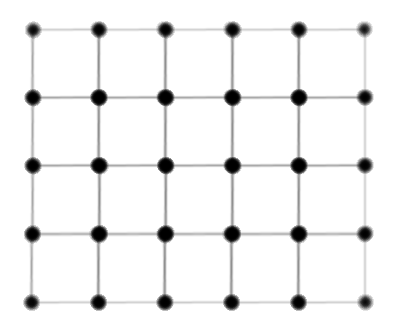
\includegraphics[scale=0.5]{fig1}
 \caption{The Graph}
\end{figure}

\begin{figure}[p]
 \centering
 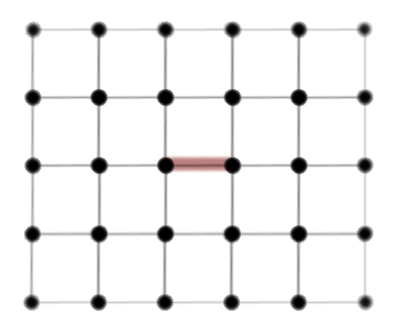
\includegraphics[scale=0.5]{fig2}
 \caption{The First Move}
\end{figure}

\begin{figure}[p]
 \centering
 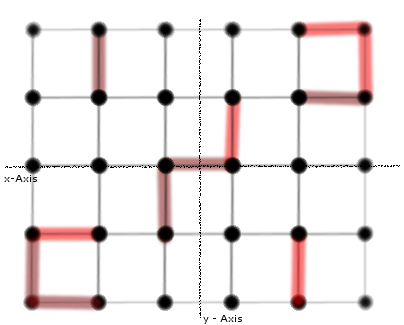
\includegraphics[scale=0.5]{fig3}
 \caption{Mirrored moves}
\end{figure}

\begin{figure}[p]
 \centering
 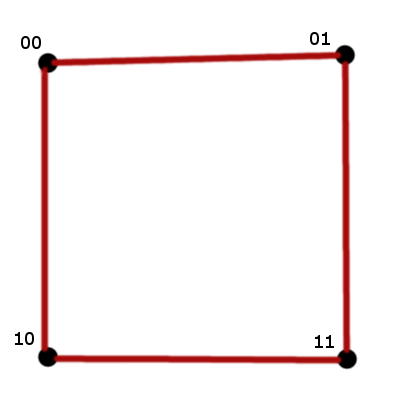
\includegraphics[scale=0.5]{fig6}
 \caption{Base Case Binary Strings}
\end{figure}

\begin{figure}[p]
 \centering
 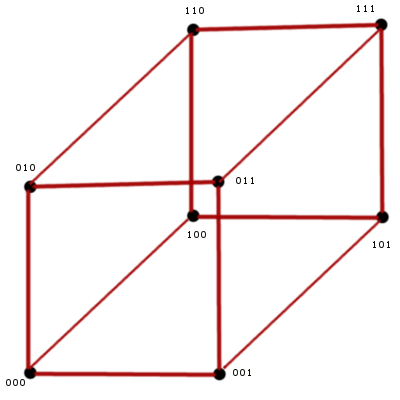
\includegraphics[scale=0.5]{fig7}
 \caption{Base Case + 1}
\end{figure}

\begin{figure}[p]
 \centering
 
\includegraphics[scale=0.5]{stn}
 \caption{Space Station}
\end{figure}

\begin{figure}[p]
 \centering
 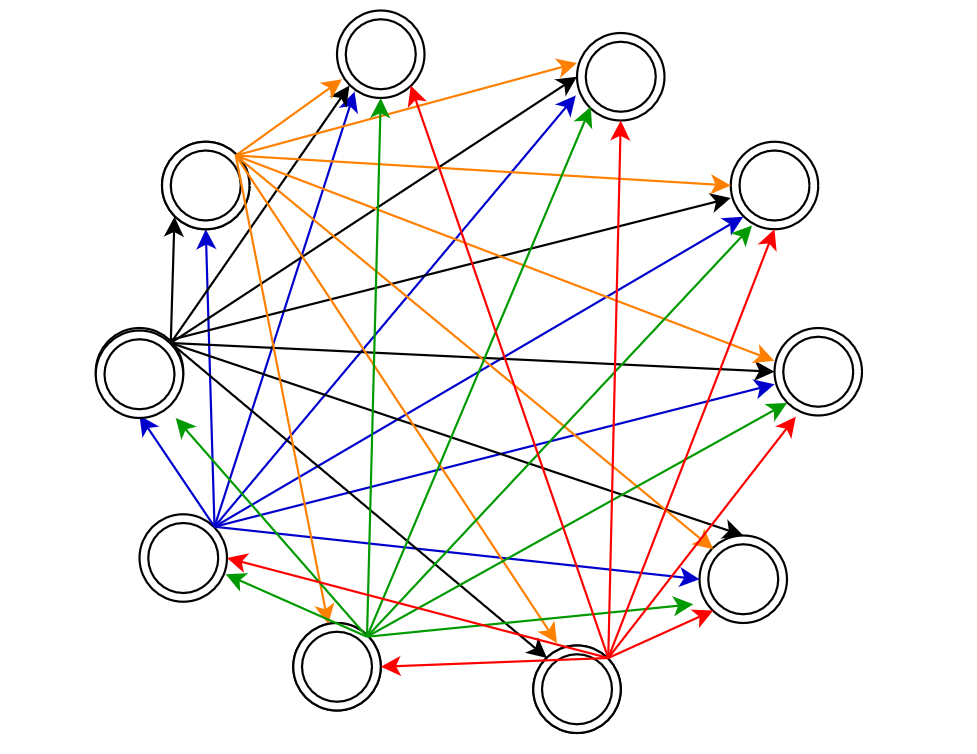
\includegraphics[scale=0.5]{fig4}
 \caption{Five Winners}
\end{figure}

\begin{figure}[p]
 \centering
 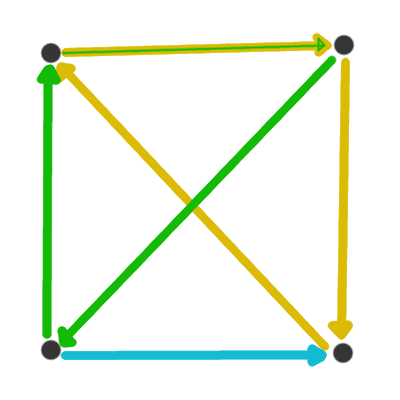
\includegraphics[scale=0.5]{fig8}
 \caption{Directed Graph n = 4}
\end{figure}

\end{document}